\section{Shape Detection}
\label{sec:shape_detection}

\subsection{Basics}

\textbf{\textcolor{blue}{Question 1:}} Remind the principle of pseudo-inverse approach.

\textit{Now you observe a positions of an asteroid at different times, and the objective is to estimate its trajectory.}

\textbf{\textcolor{blue}{Question 2:}} Complete the program \texttt{'AsteroidTry'} to estimate the asteroid trajectory. Detail the theoretical approach.

\subsubsection{Principles of the Pseudo-Inverse approach}

The pseudo-inverse approach can be applied to find the best fit models to data. This is works well for linear models, such as 
\begin{equation}
    \Vec{y} = a \vec{x} + b 
\end{equation}
where $\vec{x} = (x_1, \dots, x_n)$ and $\vec{y} = (y_1, \dots, y_n)$ are our data points and $a$ and $b$ are the sought after parameters. The linear equation can be rewritten in matrix form for each data point as
\begin{equation}
    \underbrace{\begin{pmatrix}
        y_1 \\
        \vdots \\
        y_n
    \end{pmatrix}}_{Y}
    =
    \underbrace{\begin{pmatrix}
        x_1 & 1 \\
        \vdots & \vdots \\
        x_n & 1
    \end{pmatrix}}_{X}
    \underbrace{\begin{pmatrix}
        a \\ b
    \end{pmatrix}}_{P}
\end{equation}

The parameter vector is then found by inverting the equation to 
\begin{equation}
    P = X' Y 
\end{equation}

An alternative way to formulate the problem, which is handy when the equations aren't linear, is to write it out a linear relationship as follows:
\begin{equation}
    a\vec{x} + b\vec{y} + c = 0 \Leftrightarrow -\frac{a}{c} \vec{x} - \frac{b}{c} \vec{y} = 1 \equiv \alpha \vec{x} + \beta \vec{y} = 1 
\end{equation}

The matrix form is then expressed as
\begin{equation}
    \begin{pmatrix}
        x_1 & y_1 \\
        \vdots & \vdots \\
        x_n & y_n 
    \end{pmatrix} 
    \begin{pmatrix}
        \alpha \\
        \beta
    \end{pmatrix}
    = \mathbb{1} 
    \Leftrightarrow
    X P = \mathbb{1}
\end{equation}

The pseudo-inverse is then defined by multiplying by the transpose of $X$ on both sides, before inverting the equation:
\begin{equation}
    X^t X P = X^t \mathbb{1} \Rightarrow P = (X^t X)^{-1} X^t \mathbb{1}
\end{equation}
where the $pinv(X) = (X^t X)^{-1} X^t$ is the pseudo-inverse of $X$. With this formulation, more complex models that involve powers of $x$ and $y$ can be used to fit data. For example, an asteroid's trajectory is an ellipse, whose mathematical model is given by the expression
\begin{equation}
    a x^2 + 2 b x y + c y^2 + d x + e y = 1
    \label{eq:conicSectionRotated}
\end{equation}
Here we have both linear and quadratic terms, as well as cross-terms, which describe the overall shape and orientation of the ellipse. Each term is also not independent from each other, and we can reconstruct $d$ and $e$ from $a$, $b$ and $c$. Still, the pseudo-inverse can be constructed by arranging the terms in the matrix as follows:
\begin{equation}
    \begin{pmatrix}
        x_1^2  & 2 x_1 y_1 & y_1^2  & x_1    & y_1 \\
        \vdots & \vdots    & \vdots & \vdots & \vdots \\
        x_n^2  & 2 x_n y_n & y_n^2  & x_n    & y_n \\
    \end{pmatrix}
    \begin{pmatrix}
        a \\ b \\ c \\ d \\ e 
    \end{pmatrix} = \mathbb{1} 
\end{equation}

\subsubsection{Estimation of an asteroid's trajectory}

The well-known formula for an ellipse is given as
\begin{equation}
    \frac{(x - x_0)^2}{a^2} + \frac{(y - y_0)^2}{b^2} = 1
    \label{eq:ellipse}
\end{equation}

This however does not account for the rotation of an ellipse. The parameters we get out of the pseudo inverse approach are for the rotated ellipse. We can consider the ellipse to be the rotation of a traditional, axis-aligned ellipse, that was rotated through the transformation
\begin{equation}
    \begin{cases}
        x = x'\cos\theta - y'\sin\theta \\
        y = x'\sin\theta + y'\cos\theta
    \end{cases}
    \label{eq:conicSectionTransform}
\end{equation}

This ellipse's conic section equation won't have any cross terms which arise from the rotation. That is, we expect the form
\begin{equation}
    a'x'^2 + c'y'^2 + d'x' + e'y' = 1
    \label{eq:conicSectionUnrotated}
\end{equation}

If we plug the transforms \autoref{eq:conicSectionTransform} into \autoref{eq:conicSectionRotated}, we obtain the relations between the old and new coefficients as follows:
\begin{equation}
    \begin{cases}
        a' = a \cos^2\theta + b \cos\theta\sin\theta + c\sin^2\theta \\
        b' = b (\cos^2\theta - \sin^2\theta) + 2\cos\theta\sin\theta (c-a) \\
        c' = a \sin^2\theta - b \cos\theta\sin\theta + c\cos^2\theta \\
        d' = d\cos\theta + e\sin\theta \\
        e' = -d\sin\theta + e\cos\theta 
    \end{cases}
\end{equation}

We can immediately recover the angle of rotation by imposing
\begin{equation}
    b \overset{!}{=} 0 \Leftrightarrow \frac{2b}{a - c} = \frac{2\cos\theta\sin\theta}{\cos^2\theta - \sin^2\theta}
\end{equation}

One can apply the trigonometric identity $\tan(2\theta) = \frac{2\tan\theta}{1 - \tan^2\theta}$ to find that
\begin{equation}
    \theta = \frac{1}{2} \arctan \left( \frac{2b}{a - c} \right)
\end{equation}

Next we can factorize \autoref{eq:conicSectionUnrotated} to make the traditional ellipse equation appear. By expanding the square, we obtain
\begin{equation}
    a' \left[ x' + \frac{d'}{2a'}\right]^2 + c' \left[ y' + \frac{e'}{2c'}\right]^2 = 1 + \frac{d'^2}{4 a'} + \frac{e'^2}{4 c'}
\end{equation}

From this we can read off the values of the semi-major and semi-minor axes compared to \autoref{eq:ellipse}, which will be the maximum and minimum respectively of the set 
\begin{equation}
    \left\{ \sqrt{\frac{1 + \frac{d'^2}{4 a'} + \frac{e'^2}{4 c'}}{a'}}, \sqrt{\frac{1 + \frac{d'^2}{4 a'} + \frac{e'^2}{4 c'}}{c'}}  \right\} 
\end{equation}

The center of the ellipse is trivially
\begin{equation}
    \begin{cases}
        x_0' = -\frac{d'}{2a'} \\
        y_0' = -\frac{e'}{2c'}
    \end{cases}
\end{equation}
Which must of course be rotated back into place with \autoref{eq:conicSectionTransform} to have the center point of the rotated ellipse.

With the mathematical framework at hand, the result of the MatLab implementation is shown in \autoref{fig:ReconstructedAsteroidTrajectory}. The asteroid's trajectory is generated at random every time the script is run, and the fit shows a very good match to the original trajectory.
\begin{figure}[!ht]
    \centering
    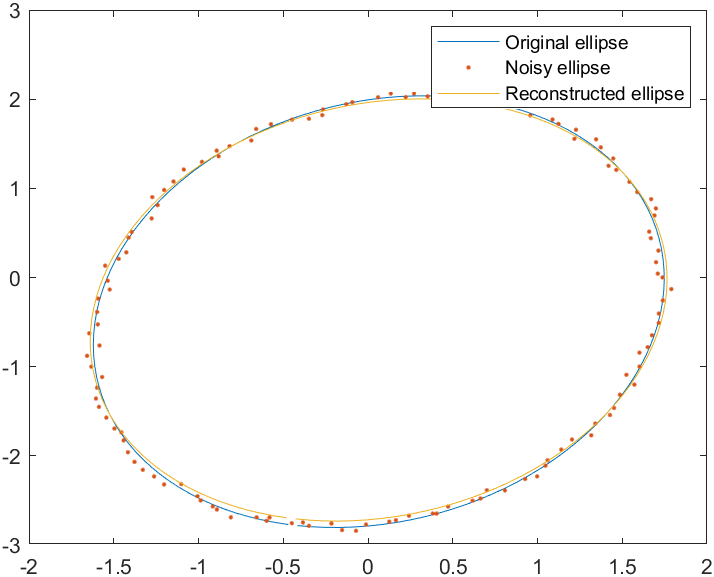
\includegraphics[width=0.5\textwidth]{Doc/Graphics/Part3/ReconstructedAsteroidTrajectory.png}
    \caption{Reconstructed asteroid trajectory}
    \label{fig:ReconstructedAsteroidTrajectory}
\end{figure}
\FloatBarrier

\subsection{Shape-Based Approaches}

\textbf{\textcolor{blue}{Question 3:}} Recall basic principle of shape detection in Computer Vision.

Now, let us consider one planet to be detected and characterised (Fig. 1) in 3 different configurations.

\textbf{\textcolor{blue}{Question 4:}} Detect \& Characterise (position, size) the 1st planet in Conf. 1.

\textbf{\textcolor{blue}{Question 5:}} What’s happen with Conf. 2 and Conf. 3?

The underlying idea is to search a pre-defined shape, which is usually a good approximation of the object we are searching for. In our case, we look for disks, which are good approximations for planets and moons. With the defined shape, we must apply an optimization algorithm, which computes the overlap between the shape's dimensions and positions and the objects in the image, and iterates until a maximum overlap is found. We apply the algorithm to the pictures shown in \autoref{fig:RecognitionShapeMoon}, \autoref{fig:RecognitionShapeJupiterEarth} and \autoref{fig:RecognitionShapeJupiterPartial}.

While the recognition of a perfect disk, such as for the moon, is very good, we can already see the flaws of this recognition method. As soon as there is more than one object, the method is biased to the larger one, as it will yield a larger overlap value in terms of pixel numbers; additionally, the method is also searching for a single object only, and doesn't try to fit multiple disks. The method also breaks down as soon as the planet is not fully illuminated and has a croissant shape instead of a circle, which leads to a significant mis-estimation of the objects shape.  

\begin{figure}[!ht]
    \centering
    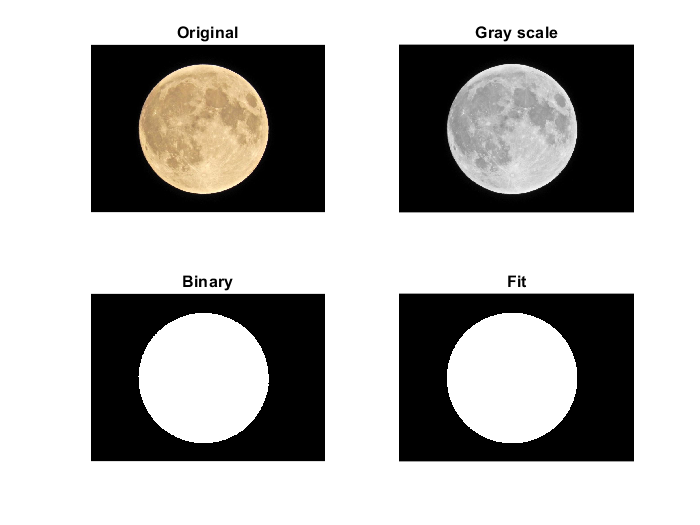
\includegraphics[width=0.75\linewidth]{Doc/Graphics/Part3/fit_moon.png}
    \caption{Shape approach on the Moon image}
    \label{fig:RecognitionShapeMoon}
\end{figure}
\begin{figure}[!ht]
    \centering
    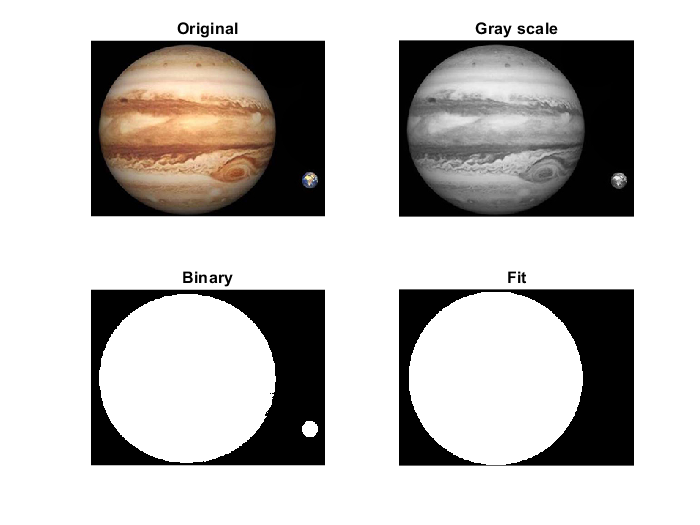
\includegraphics[width=0.75\linewidth]{Doc/Graphics/Part3/fit_jupiter_earth.png}
    \caption{Shape approach on the Jupiter and Earth image}
    \label{fig:RecognitionShapeJupiterEarth}
\end{figure}
\begin{figure}[!ht]
    \centering
    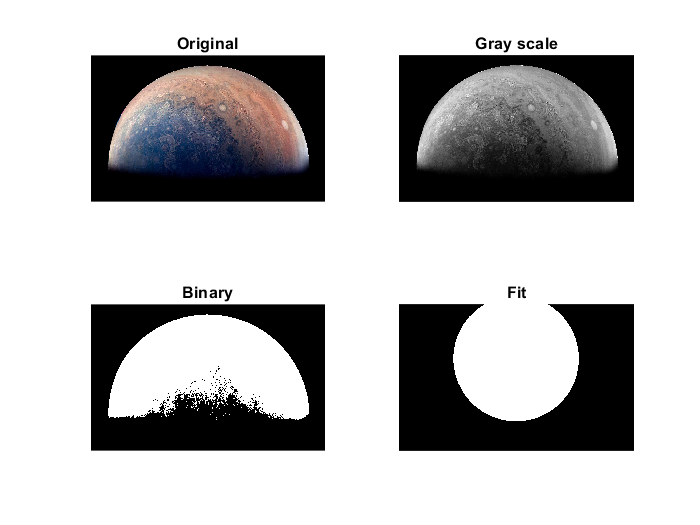
\includegraphics[width=0.75\linewidth]{Doc/Graphics/Part3/fit_jupiter_partial.png}
    \caption{Shape approach on the partial Jupiter image}
    \label{fig:RecognitionShapeJupiterPartial}
\end{figure}
\FloatBarrier




\subsection{Contour-Based Approaches}

\textbf{\textcolor{blue}{Question 6:}} Extract the planet (Conf. 1) using N points and next a Pseudo-Inverse Approach. What’s happen in other configurations?

\textbf{\textcolor{blue}{Question 7:}} Same as 6.

\textbf{\textcolor{blue}{Question 8:}} Extract the planet (Conf. 1) using an Optimisation algorithm. What’s happen in other configurations?

\textbf{\textcolor{blue}{Question 9:}} Explain the RANSAC Algorithm. Use it in Conf. 2 and Conf. 3.

\textbf{\textcolor{blue}{Question 10:}} Compare with the circular Hough Transform.

\subsubsection{Pseudo-inverse Approach}

Circle equation:
\begin{equation}
    (x-x_0)^2 + (y-y_0)^2 = r^2
\end{equation}

As conic section:
\begin{equation}
    A(x^2+y^2) + Bx + Cy = 1
\end{equation}

Similarly to the ellipse, we recover the center coordinates by expanding the square, and the radius  by comparing with the traditional circle equation:
\begin{equation}
    \begin{cases}
        x_0 = \frac{-B}{2A} \\[10pt]
        y_0 = \frac{-C}{2A} \\[10pt]
        r = \sqrt{\frac{1}{A} + \left(\frac{B}{2A}\right)^2 +\left(\frac{C}{2A}\right)^2} = \sqrt{\frac{1}{A} + x_0^2 + y_0^2} &
    \end{cases}
\end{equation}

Pseudo-inverse formulation
\begin{equation}
    \begin{pmatrix}
        x_1^2 + y_1^2 & x_1 & y_1 \\
        \vdots & \vdots & \vdots \\
        x_n^2 + y_n^2 & x_n & y_n 
    \end{pmatrix}
    \begin{pmatrix}
        A \\ B \\ C 
    \end{pmatrix}
    = \mathbb{1}
\end{equation}

To apply the method, we must first extract the edges of the image, which we do by applying a laplacian filter kernel. This method yields the outer of the objects, which is exactly what we want.

\begin{figure}[!ht]
    \centering
    \begin{subfigure}{0.32\textwidth}
        \centering
        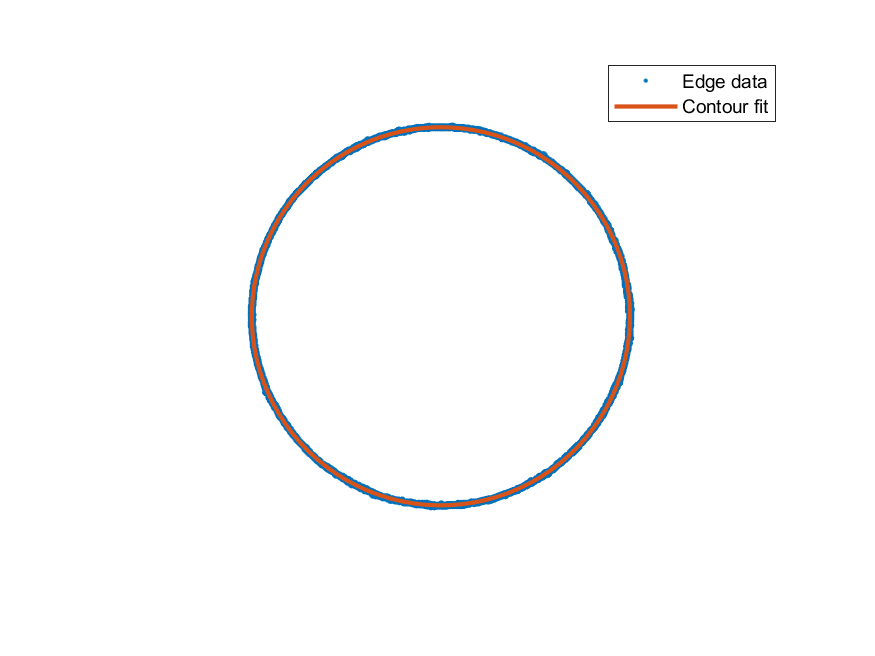
\includegraphics[width=\textwidth]{Doc/Graphics/Part3/contourDection_pseudoInverse_moon.png}
        \caption{Full Moon}
    \end{subfigure}
    \begin{subfigure}{0.32\textwidth}
        \centering
        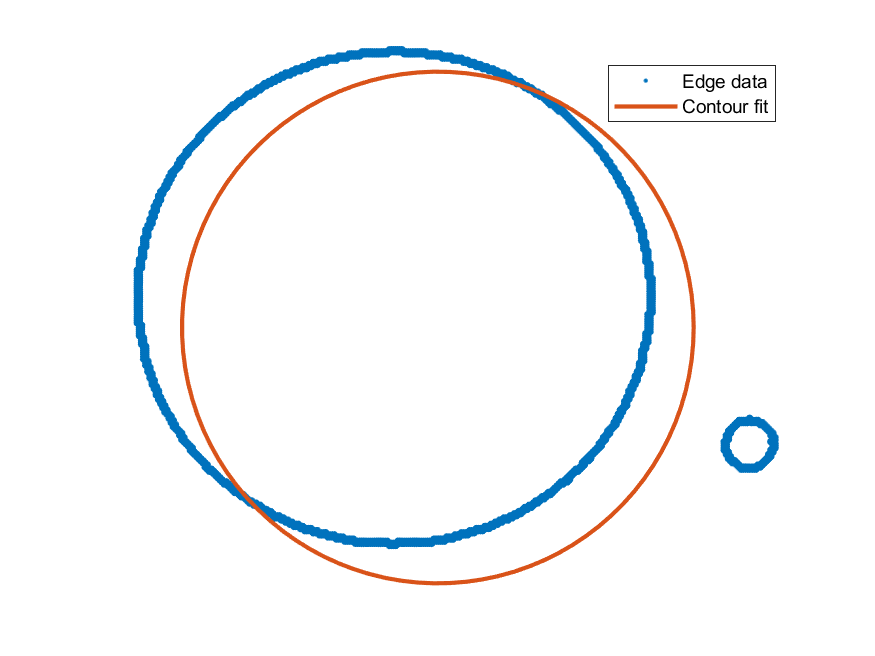
\includegraphics[width=\textwidth]{Doc/Graphics/Part3/contourDection_pseudoInverse_jupiter_earth.png}
        \caption{Jupiter and Earth}
    \end{subfigure}
    \begin{subfigure}{0.32\textwidth}
        \centering
        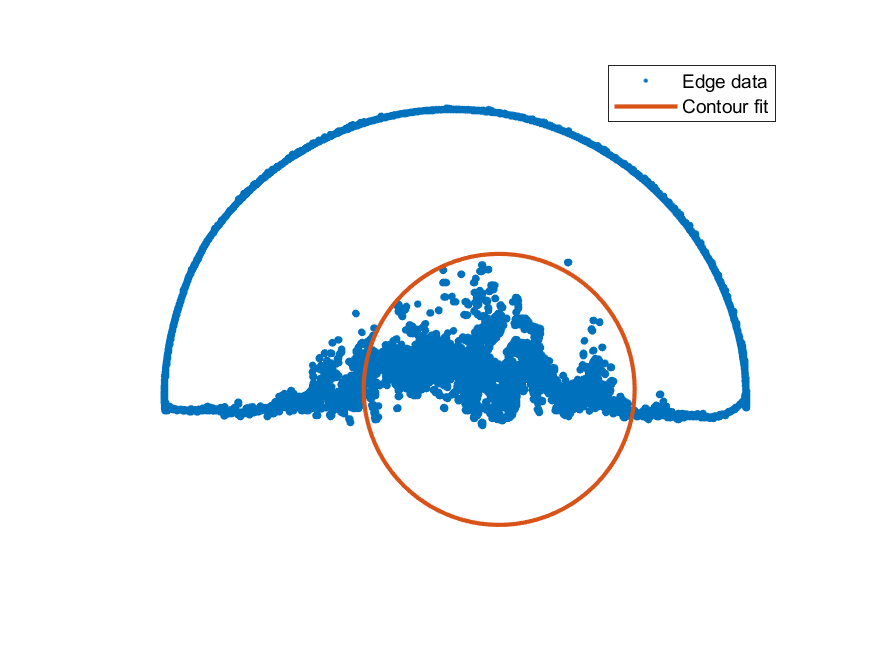
\includegraphics[width=\textwidth]{Doc/Graphics/Part3/contourDection_pseudoInverse_jupiter_partial.png}
        \caption{Jupiter croissant}
    \end{subfigure}
    \caption{Contour approach and pseudo-inverse method results}
    \label{fig:enter-label}
\end{figure}

We can observe again, that the method is excellent for the full moon, which has the exact shape we are trying to fit. When there is more than one object, the fit is biased towards what seems to be the center of mass of the system. In the case of a partial shape the method breaks down again because of all the noise and the fact that it tries to take all data points into account.

\subsubsection{Optimization approach}

With this approach, we use MatLab's optimization function to search for the minimum in a quadratic cost function, which is simply the sum of the errors of the fit. Interestingly, the optimization works well on the first two configurations. The fact that it fits nicely on Jupiter, but not Earth, is that the optimization method is subject to finding local minima. There is two of such points which correspond to the two planets. Finally on Jupiter's croissant, the method doesn't work at all, as there is to many points which do not correspond to the circumference of the circle, but the algorithm still treats equally important. This results in the fit going through the 'noise' moreso than through the actual points we are interested.

\begin{figure}[!ht]
    \centering
    \begin{subfigure}{0.32\textwidth}
        \centering
        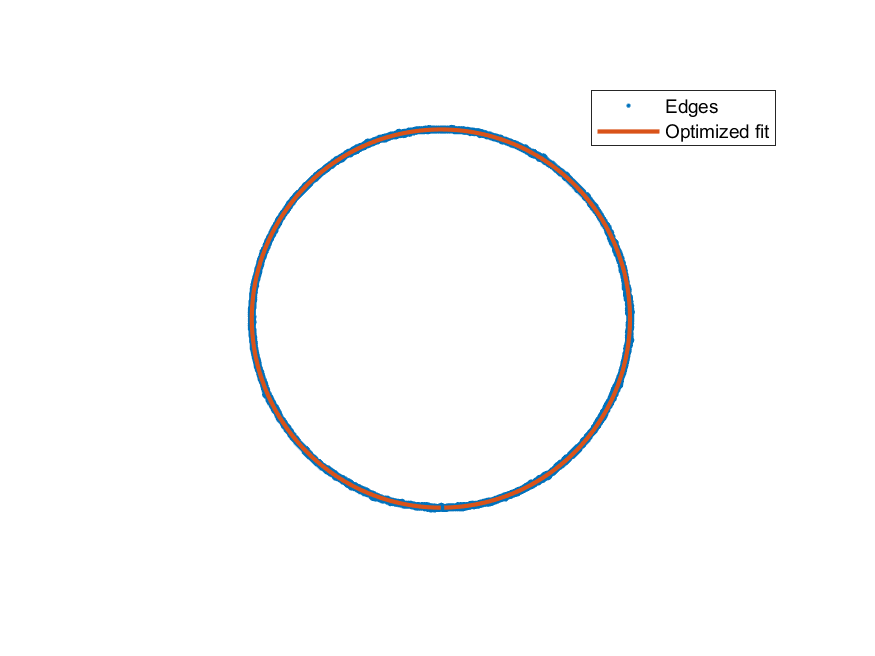
\includegraphics[width=\textwidth]{Doc/Graphics/Part3/Optimization_moon.png}
        \caption{Full Moon}
    \end{subfigure}
    \hfill
    \begin{subfigure}{0.32\textwidth}
        \centering
        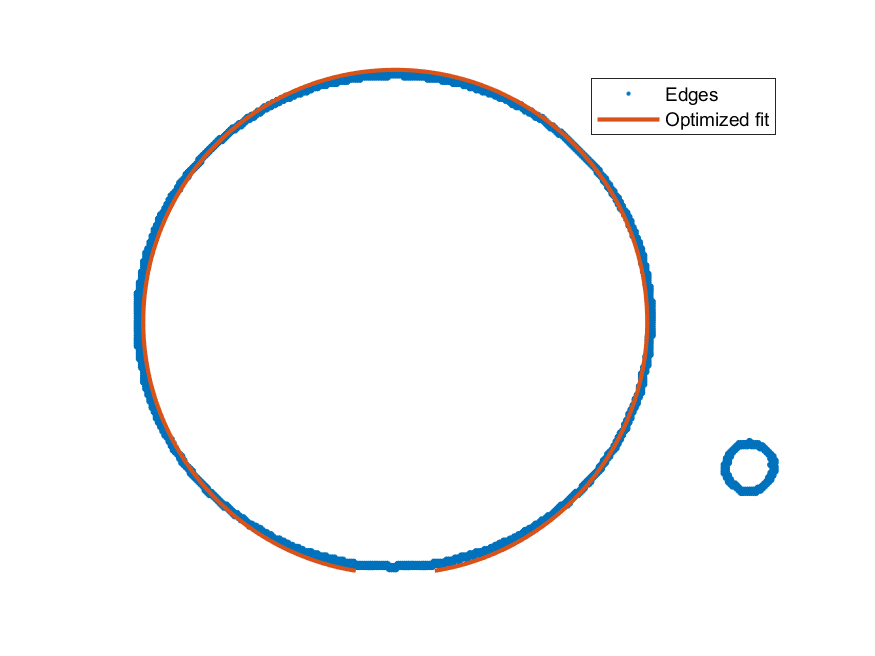
\includegraphics[width=\textwidth]{Doc/Graphics/Part3/Optimization_jupiter_earth.png}
        \caption{Jupiter and Earth}
    \end{subfigure}
    \hfill
    \begin{subfigure}{0.32\textwidth}
        \centering
        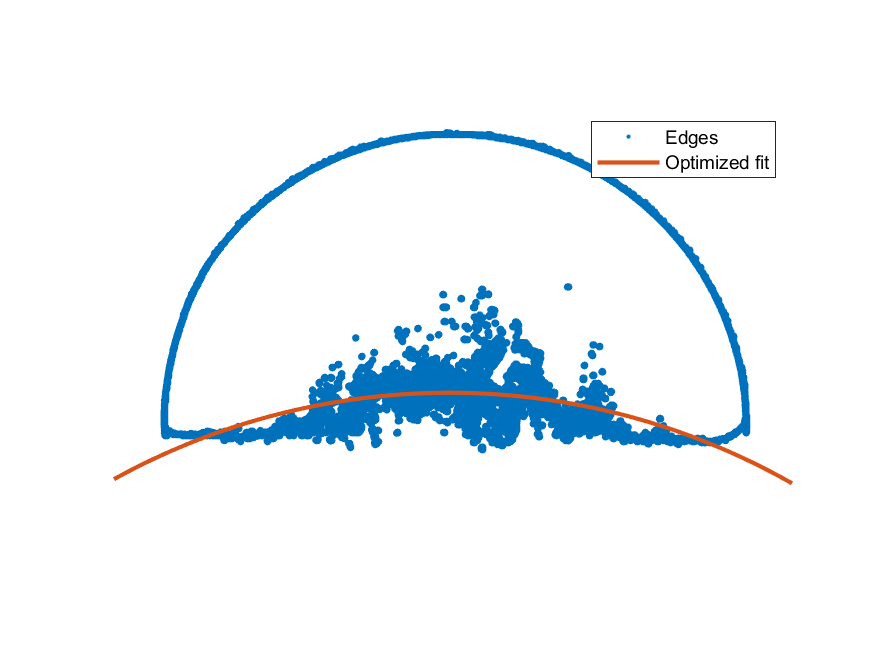
\includegraphics[width=\textwidth]{Doc/Graphics/Part3/Optimization_jupiter_partial.png}
        \caption{Jupiter croissant}
    \end{subfigure}
    \caption{Optimization approach results}
    \label{fig:enter-label}
\end{figure}

\subsubsection{RANSAC approach}

The goal of the \textbf{RAN}dom \textbf{SA}mple \textbf{C}onsensus (RANSAC) algorithm is to identify only the points which are actually correspond to the thing we are interested in. Therefore we can define 'inliers' and 'outlier' data points which have get sifted through. When trying to fit a circle, we have to define a tolerance region around the line of best fit, which defines the boundary between the inliers and outliers. A minimum amount of points to be fitted must also be specified, so that we do not under-fit the data, potentially fitting on noise. The algorithm is built in a way that it generates multiple fit solutions based on randomized start conditions, of which the best solution must be selected by the end. This is decided based on either inlier count or least error.

The steps of the algorithm (for fitting circles) are as follows:
\begin{enumerate}
    \item Select 3 data points randomly (minimum to uniquely identify a circle)
    \item Fit the model to these points
    \item Identify the inliers based on the threshold
    \item If the inlier count is less than the minimum allowed, go back to step 1
    \item Fit the model using all the identified inliers
    \item Identify the inliers based on the threshold
    \item If the inlier count is less than the minimum allowed, go back to step 1
    \item Determine the error of the candidate model fit
    \item Add the fit, the inlier count and error to the list of candidate model fits.
    \item Repeat until the maximum allowed iteration number
    \item Examine the list of candidate fits and select the one with highest point number, and/or least error
\end{enumerate}

The results are shown in \autoref{fig:resultsRansac}. We can see that the model is excellent at fitting noisy data, as is the case for the Jupiter croissant. In the case of the Jupiter-Earth image, it also successfully excludes the Earth from the fit. The minimum number of inliers to be considered is based on the total amount of data points in the image, and is subject to tuning. The tolerances for identifying inliers also need tweaking through some trial-and error until an optimal fit is found. This leads to certain sets of input parameters to yield no results.
\begin{figure}[!ht]
    \centering
    \begin{subfigure}{0.32\textwidth}
        \centering
        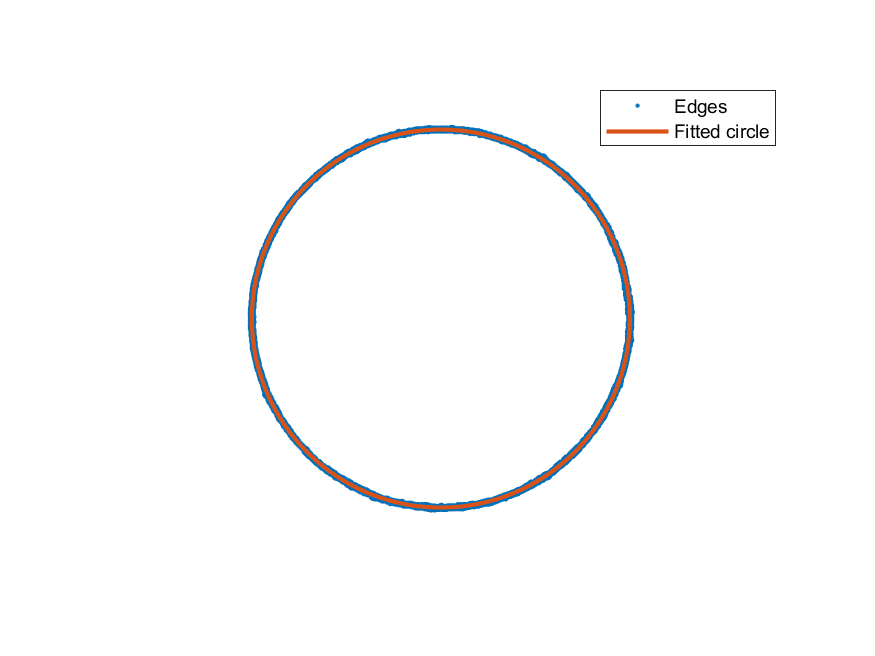
\includegraphics[width=\textwidth]{Doc/Graphics/Part3/RANSAC_moon.png}
        \caption{Full Moon}
    \end{subfigure}
    \hfill
    \begin{subfigure}{0.32\textwidth}
        \centering
        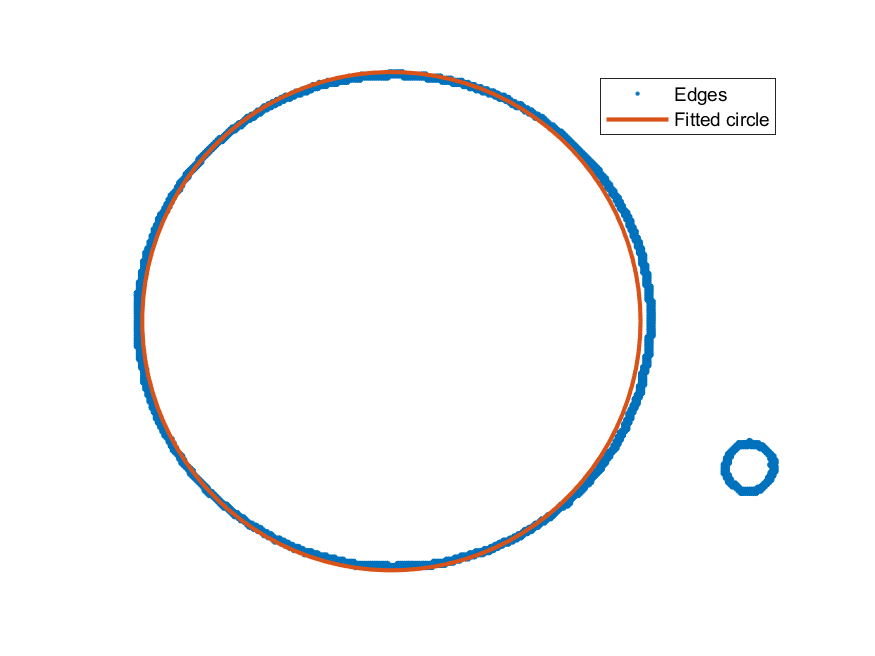
\includegraphics[width=\textwidth]{Doc/Graphics/Part3/RANSAC_jupiter_earth.png}
        \caption{Jupiter and Earth}
    \end{subfigure}
    \hfill
    \begin{subfigure}{0.32\textwidth}
        \centering
        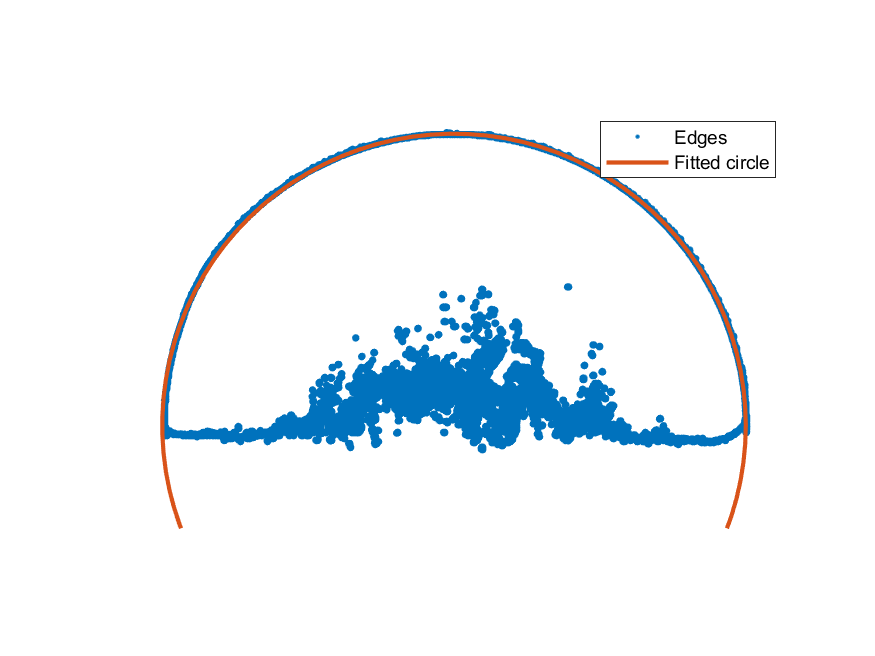
\includegraphics[width=\textwidth]{Doc/Graphics/Part3/RANSAC_jupiter_partial.png}
        \caption{Jupiter croissant}
    \end{subfigure}
    \caption{RANSAC approach results}
    \label{fig:resultsRansac}
\end{figure}

\subsubsection{Circular Hough transform approach}

The circle Hough transform works by examining the image in the Hough parameter space to identify possible circular features. It requires either the radius or range of values of radii of the circles to be known. MatLab has a built-in method for this: \texttt{imfindcircles()}. While it works on colored and grayscale images, the results seem best when the image is binarized, as the method won't be as sensitive to shapes on the surface, as can be seen in \autoref{fig:resultsHough}. The method seems rather inconsistent overall, and requires a lot of tuning to get right. It seems to detect circles where there aren't any visible features to the human eye, which might be due to slight shadows. It is however able to detect both planets at once in the Jupiter-Earth configuration.

\begin{figure}[!ht]
    \centering
    \begin{subfigure}{0.49\textwidth}
        \centering
        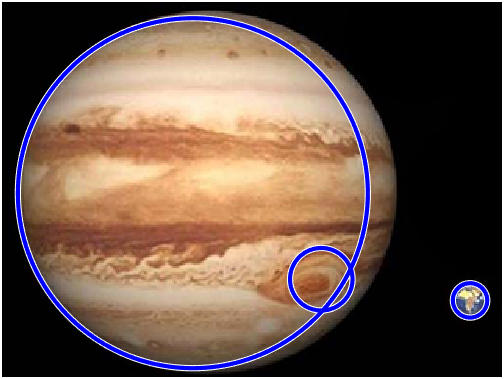
\includegraphics[width=\textwidth]{Doc/Graphics/Part3/hough_rgb_S085_TwoStage.png}
        \caption{0.85 Sensitivity, Two Stage Method}
    \end{subfigure}
    \hfill
    \begin{subfigure}{0.49\textwidth}
        \centering
        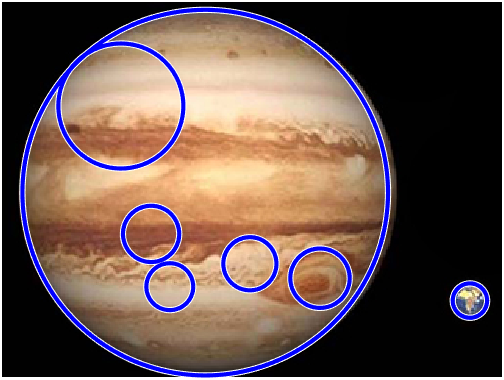
\includegraphics[width=\textwidth]{Doc/Graphics/Part3/hough_rgb_S09_TwoStage.png}
        \caption{0.9 Sensitivity, Two Stage Method}
    \end{subfigure}
    \begin{subfigure}{0.49\textwidth}
        \centering
        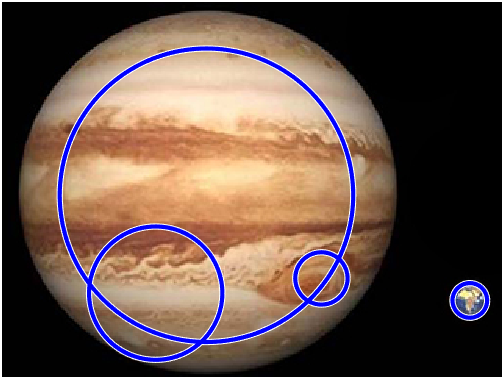
\includegraphics[width=\textwidth]{Doc/Graphics/Part3/hough_rgb_S09_PhaseCode.png}
        \caption{0.9 Sensitivity, Phase Code Method}
    \end{subfigure} 
    \hfill
    \begin{subfigure}{0.49\textwidth}
        \centering
        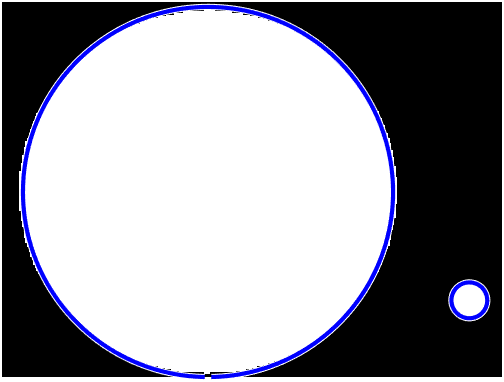
\includegraphics[width=\textwidth]{Doc/Graphics/Part3/hough_bw.png}
        \caption{Default parameters on binary image}
    \end{subfigure}    
    \caption{Hough Method results}
    \label{fig:resultsHough}
\end{figure}